\PassOptionsToPackage{unicode=true}{hyperref} % options for packages loaded elsewhere
\PassOptionsToPackage{hyphens}{url}
%
\documentclass[]{article}
\usepackage{lmodern}
\usepackage{amssymb,amsmath}
\usepackage{ifxetex,ifluatex}
\usepackage{fixltx2e} % provides \textsubscript
\ifnum 0\ifxetex 1\fi\ifluatex 1\fi=0 % if pdftex
  \usepackage[T1]{fontenc}
  \usepackage[utf8]{inputenc}
  \usepackage{textcomp} % provides euro and other symbols
\else % if luatex or xelatex
  \usepackage{unicode-math}
  \defaultfontfeatures{Ligatures=TeX,Scale=MatchLowercase}
\fi
% use upquote if available, for straight quotes in verbatim environments
\IfFileExists{upquote.sty}{\usepackage{upquote}}{}
% use microtype if available
\IfFileExists{microtype.sty}{%
\usepackage[]{microtype}
\UseMicrotypeSet[protrusion]{basicmath} % disable protrusion for tt fonts
}{}
\IfFileExists{parskip.sty}{%
\usepackage{parskip}
}{% else
\setlength{\parindent}{0pt}
\setlength{\parskip}{6pt plus 2pt minus 1pt}
}
\usepackage{hyperref}
\hypersetup{
            pdftitle={Summer Research Project: Bats},
            pdfborder={0 0 0},
            breaklinks=true}
\urlstyle{same}  % don't use monospace font for urls
\usepackage[margin=1in]{geometry}
\usepackage{color}
\usepackage{fancyvrb}
\newcommand{\VerbBar}{|}
\newcommand{\VERB}{\Verb[commandchars=\\\{\}]}
\DefineVerbatimEnvironment{Highlighting}{Verbatim}{commandchars=\\\{\}}
% Add ',fontsize=\small' for more characters per line
\usepackage{framed}
\definecolor{shadecolor}{RGB}{248,248,248}
\newenvironment{Shaded}{\begin{snugshade}}{\end{snugshade}}
\newcommand{\AlertTok}[1]{\textcolor[rgb]{0.94,0.16,0.16}{#1}}
\newcommand{\AnnotationTok}[1]{\textcolor[rgb]{0.56,0.35,0.01}{\textbf{\textit{#1}}}}
\newcommand{\AttributeTok}[1]{\textcolor[rgb]{0.77,0.63,0.00}{#1}}
\newcommand{\BaseNTok}[1]{\textcolor[rgb]{0.00,0.00,0.81}{#1}}
\newcommand{\BuiltInTok}[1]{#1}
\newcommand{\CharTok}[1]{\textcolor[rgb]{0.31,0.60,0.02}{#1}}
\newcommand{\CommentTok}[1]{\textcolor[rgb]{0.56,0.35,0.01}{\textit{#1}}}
\newcommand{\CommentVarTok}[1]{\textcolor[rgb]{0.56,0.35,0.01}{\textbf{\textit{#1}}}}
\newcommand{\ConstantTok}[1]{\textcolor[rgb]{0.00,0.00,0.00}{#1}}
\newcommand{\ControlFlowTok}[1]{\textcolor[rgb]{0.13,0.29,0.53}{\textbf{#1}}}
\newcommand{\DataTypeTok}[1]{\textcolor[rgb]{0.13,0.29,0.53}{#1}}
\newcommand{\DecValTok}[1]{\textcolor[rgb]{0.00,0.00,0.81}{#1}}
\newcommand{\DocumentationTok}[1]{\textcolor[rgb]{0.56,0.35,0.01}{\textbf{\textit{#1}}}}
\newcommand{\ErrorTok}[1]{\textcolor[rgb]{0.64,0.00,0.00}{\textbf{#1}}}
\newcommand{\ExtensionTok}[1]{#1}
\newcommand{\FloatTok}[1]{\textcolor[rgb]{0.00,0.00,0.81}{#1}}
\newcommand{\FunctionTok}[1]{\textcolor[rgb]{0.00,0.00,0.00}{#1}}
\newcommand{\ImportTok}[1]{#1}
\newcommand{\InformationTok}[1]{\textcolor[rgb]{0.56,0.35,0.01}{\textbf{\textit{#1}}}}
\newcommand{\KeywordTok}[1]{\textcolor[rgb]{0.13,0.29,0.53}{\textbf{#1}}}
\newcommand{\NormalTok}[1]{#1}
\newcommand{\OperatorTok}[1]{\textcolor[rgb]{0.81,0.36,0.00}{\textbf{#1}}}
\newcommand{\OtherTok}[1]{\textcolor[rgb]{0.56,0.35,0.01}{#1}}
\newcommand{\PreprocessorTok}[1]{\textcolor[rgb]{0.56,0.35,0.01}{\textit{#1}}}
\newcommand{\RegionMarkerTok}[1]{#1}
\newcommand{\SpecialCharTok}[1]{\textcolor[rgb]{0.00,0.00,0.00}{#1}}
\newcommand{\SpecialStringTok}[1]{\textcolor[rgb]{0.31,0.60,0.02}{#1}}
\newcommand{\StringTok}[1]{\textcolor[rgb]{0.31,0.60,0.02}{#1}}
\newcommand{\VariableTok}[1]{\textcolor[rgb]{0.00,0.00,0.00}{#1}}
\newcommand{\VerbatimStringTok}[1]{\textcolor[rgb]{0.31,0.60,0.02}{#1}}
\newcommand{\WarningTok}[1]{\textcolor[rgb]{0.56,0.35,0.01}{\textbf{\textit{#1}}}}
\usepackage{graphicx,grffile}
\makeatletter
\def\maxwidth{\ifdim\Gin@nat@width>\linewidth\linewidth\else\Gin@nat@width\fi}
\def\maxheight{\ifdim\Gin@nat@height>\textheight\textheight\else\Gin@nat@height\fi}
\makeatother
% Scale images if necessary, so that they will not overflow the page
% margins by default, and it is still possible to overwrite the defaults
% using explicit options in \includegraphics[width, height, ...]{}
\setkeys{Gin}{width=\maxwidth,height=\maxheight,keepaspectratio}
\setlength{\emergencystretch}{3em}  % prevent overfull lines
\providecommand{\tightlist}{%
  \setlength{\itemsep}{0pt}\setlength{\parskip}{0pt}}
\setcounter{secnumdepth}{0}
% Redefines (sub)paragraphs to behave more like sections
\ifx\paragraph\undefined\else
\let\oldparagraph\paragraph
\renewcommand{\paragraph}[1]{\oldparagraph{#1}\mbox{}}
\fi
\ifx\subparagraph\undefined\else
\let\oldsubparagraph\subparagraph
\renewcommand{\subparagraph}[1]{\oldsubparagraph{#1}\mbox{}}
\fi

% set default figure placement to htbp
\makeatletter
\def\fps@figure{htbp}
\makeatother


\title{Summer Research Project: Bats}
\author{}
\date{\vspace{-2.5em}}

\begin{document}
\maketitle

\begin{center}\rule{0.5\linewidth}{0.5pt}\end{center}

\hypertarget{by-randy-posada}{%
\paragraph{\texorpdfstring{\emph{By Randy
Posada}}{By Randy Posada}}\label{by-randy-posada}}

\begin{center}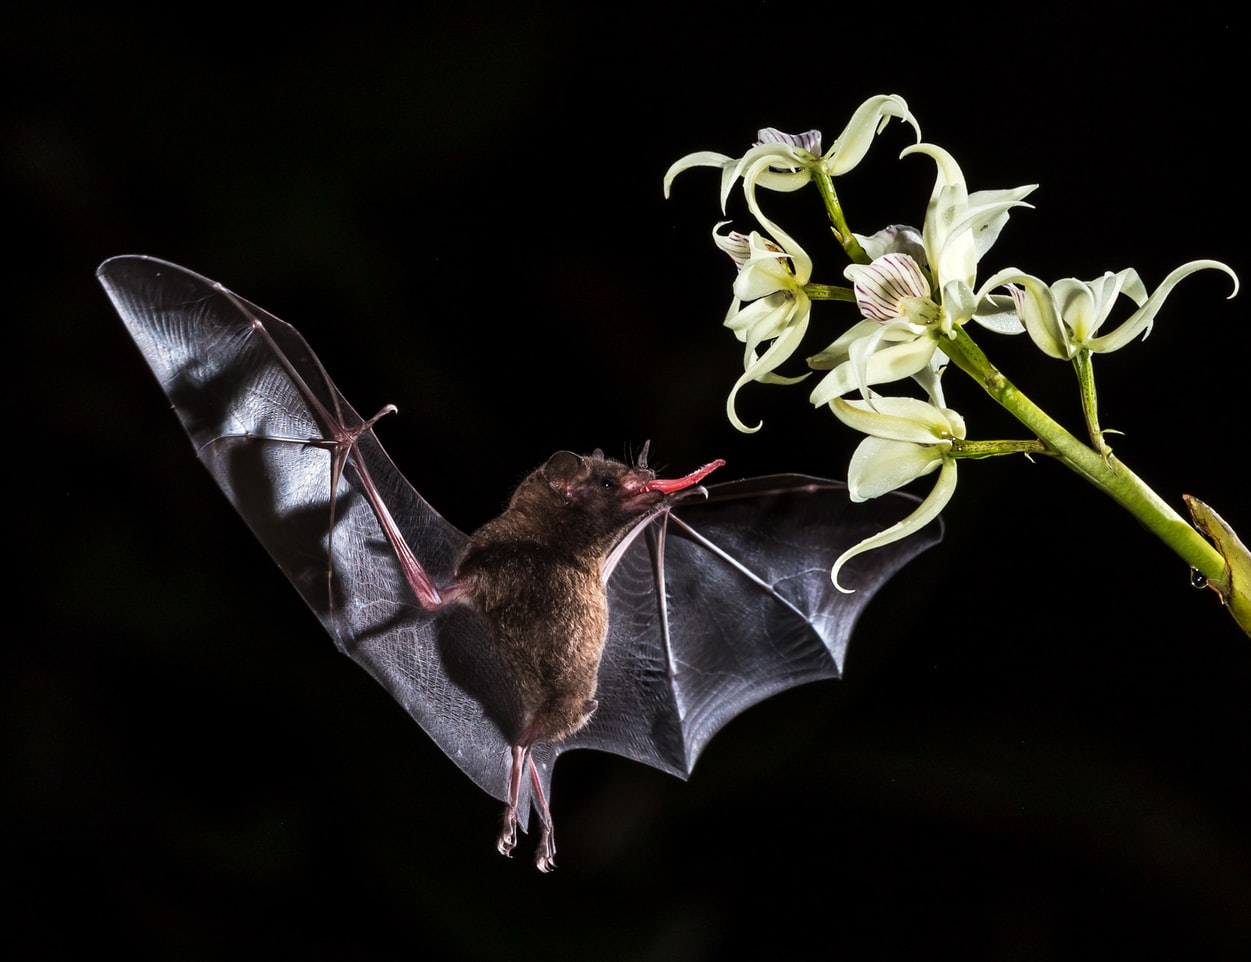
\includegraphics[width=1\linewidth,height=0.5\textheight]{../images/Batphoto1} \end{center}

\emph{Fig.cap="\protect\hyperlink{Attributions}{See attributions for
link}}

\begin{Shaded}
\begin{Highlighting}[]
\KeywordTok{getwd}\NormalTok{()}
\CommentTok{#> [1] "/Users/luna/pj_physcraper/bats/vignettes"}
\end{Highlighting}
\end{Shaded}

\begin{center}\rule{0.5\linewidth}{0.5pt}\end{center}

\hypertarget{my-report}{%
\section{\texorpdfstring{\textbf{My
Report}}{My Report}}\label{my-report}}

\hypertarget{overview}{%
\subsection{\texorpdfstring{\emph{Overview}}{Overview}}\label{overview}}

In this report I use the OpenTree of life alongside Physcraper to create
and access an updated phylogentic tree of all bats.

There are over 1000 different species of bats. These extraordinary
flying mammals use their hands to fly; granted their order name
\emph{chiroptera}, which translates in Greek to `Hand Wings'. Each of
their fingers are connected to one another through a thin layer of skin
which allows these nocturnal mammals to take off into flight. Chiroptera
are the only mammals with the capability of continued flight.

\begin{center}\rule{0.5\linewidth}{0.5pt}\end{center}

\begin{Shaded}
\begin{Highlighting}[]

\NormalTok{my_taxa <-}\StringTok{ }\KeywordTok{c}\NormalTok{(}\StringTok{"chiroptera"}\NormalTok{)}
\NormalTok{resolved_names <-}\StringTok{ }\NormalTok{rotl}\OperatorTok{::}\KeywordTok{tnrs_match_names}\NormalTok{(}\DataTypeTok{names =}\NormalTok{ my_taxa)}

\NormalTok{resolved_names}
\CommentTok{#>   search_string unique_name approximate_match ott_id is_synonym flags}
\CommentTok{#> 1    chiroptera  Chiroptera             FALSE 574724      FALSE      }
\CommentTok{#>   number_matches}
\CommentTok{#> 1              1}
\end{Highlighting}
\end{Shaded}

\begin{Shaded}
\begin{Highlighting}[]
\KeywordTok{class}\NormalTok{(resolved_names)}
\CommentTok{#> [1] "match_names" "data.frame"}
\end{Highlighting}
\end{Shaded}

\begin{Shaded}
\begin{Highlighting}[]
\NormalTok{resolved_names[}\DecValTok{1}\NormalTok{,]}
\CommentTok{#>   search_string unique_name approximate_match ott_id is_synonym flags}
\CommentTok{#> 1    chiroptera  Chiroptera             FALSE 574724      FALSE      }
\CommentTok{#>   number_matches}
\CommentTok{#> 1              1}
\end{Highlighting}
\end{Shaded}

\begin{Shaded}
\begin{Highlighting}[]
\NormalTok{resolved_names[}\DecValTok{1}\NormalTok{,}\StringTok{"unique_name"}\NormalTok{]}
\CommentTok{#> [1] "Chiroptera"}
\end{Highlighting}
\end{Shaded}

This gives all info from the current OpenTree synthetic tree

\begin{Shaded}
\begin{Highlighting}[]
\NormalTok{rotl}\OperatorTok{::}\KeywordTok{tol_about}\NormalTok{()}
\CommentTok{#> }
\CommentTok{#> OpenTree Synthetic Tree of Life.}
\CommentTok{#> }
\CommentTok{#> Tree version: opentree12.3}
\CommentTok{#> Taxonomy version: 3.2draft9}
\CommentTok{#> Constructed on: 2019-12-23 11:41:23}
\CommentTok{#> Number of terminal taxa: 2391916}
\CommentTok{#> Number of source trees: 1216}
\CommentTok{#> Number of source studies: 1162}
\CommentTok{#> Source list present: false}
\CommentTok{#> Root taxon: cellular organisms}
\CommentTok{#> Root ott_id: 93302}
\CommentTok{#> Root node_id: ott93302}
\end{Highlighting}
\end{Shaded}

This gets Chiroptera OTT id:

\begin{Shaded}
\begin{Highlighting}[]
\NormalTok{chiroptera_ott_id <-}\StringTok{ }\NormalTok{rotl}\OperatorTok{::}\KeywordTok{tnrs_match_names}\NormalTok{(}\StringTok{"Chiroptera"}\NormalTok{)}\OperatorTok{$}\NormalTok{ott_id}
\NormalTok{chiroptera_ott_id}
\CommentTok{#> [1] 574724}
\end{Highlighting}
\end{Shaded}

\begin{Shaded}
\begin{Highlighting}[]
\NormalTok{chiroptera_subtree <-}\StringTok{ }\NormalTok{rotl}\OperatorTok{::}\KeywordTok{tol_subtree}\NormalTok{(}\DataTypeTok{ott_id =}\NormalTok{ chiroptera_ott_id)}
\CommentTok{#> Warning in collapse_singles(tr, show_progress): Dropping singleton nodes with}
\CommentTok{#> labels: Murina aurata ott45655, Murina huttoni ott61865, Eudiscopus ott264809,}
\CommentTok{#> Myotis cf. nipalensis ott840249, Myotis muricola ott878677, Myotis siligorensis}
\CommentTok{#> ott687555, Myotis bombinus ott311767, Myotis myotis ott966432, Myotis bocagii}
\CommentTok{#> ott307135, Myotis nesopolus ott898241, Myotis oxyotus ott878679, Myotis}
\CommentTok{#> martiniquensis ott939105, Myotis evotis ott235790, Myotis brandtii ott353460,}
\CommentTok{#> Submyotodon ott3614201, Scotomanes ott113460, Ia ott797469, Lasionycteris}
\CommentTok{#> ott401282, Nycticeinops ott342709, Philetor ott546480, Pipistrellus javanicus}
\CommentTok{#> ott826863, Nyctalus leisleri ott342721, Plecotus teneriffae ott264117, Plecotus}
\CommentTok{#> austriacus ott1080291, Plecotus macrobullaris ott50014, Euderma ott76924,}
\CommentTok{#> Idionycteris ott401286, Perimyotis ott6146540, Parastrellus ott716687, Lasiurus}
\CommentTok{#> blossevillii ott362948, Dasypterus intermedius ott170073, Aeorestes cinereus}
\CommentTok{#> ott369537, Scotophilus viridis ott819861, Miniopterinae ott846399, Miniopterus}
\CommentTok{#> griveaudi ott584454, Miniopterus natalensis ott18887, Niumbaha ott6146535,}
\CommentTok{#> Scotozous ott3614128, Scoteanax ott3614191, Pharotis ott3614132, Mimetillus}
\CommentTok{#> ott3614192, Atalapha ott7656404, Cynomops abrasus ott1014495, Cynomops}
\CommentTok{#> paranus ott300974, Eumops glaucinus ott548118, Eumops bonariensis ott781186,}
\CommentTok{#> Sauromys ott435180, Molossus currentium ott3614007, Tomopeas ott876504,}
\CommentTok{#> Platymops ott3614012, Natalus stramineus ott579474, Nyctiellus ott120208,}
\CommentTok{#> Myzopodidae ott6788, Centurio senex ott351782, Sphaeronycteris ott116171,}
\CommentTok{#> Pygoderma ott688702, Ametrida ott688666, Ariteus ott688693, Ardops ott148558,}
\CommentTok{#> Cubanycteris ott4118392, Ectophylla ott688691, Platyrrhinus helleri ott927279,}
\CommentTok{#> Platyrrhinus lineatus ott780066, Mesophylla (genus in Opisthokonta) ott148642,}
\CommentTok{#> Sturnira lilium ott401293, Lionycteris ott1060471, Platalina ott1060470,}
\CommentTok{#> Xeronycteris ott4118394, Lophostoma silvicolum ott951266, Macrophyllum}
\CommentTok{#> ott658351, Vampyrum ott218144, Chrotopterus ott792614, Brachyphyllinae}
\CommentTok{#> ott744584, Brachyphylla nana ott179313, Lichonycteris ott269226, Musonycteris}
\CommentTok{#> ott269228, Choeronycteris ott503345, Hylonycteris ott269227, Diaemus ott792615,}
\CommentTok{#> Neonycteris ott3613611, Scleronycteris ott3613622, Dryadonycteris ott6146448,}
\CommentTok{#> Pteronotus davyi ott759858, Pteronotus personatus ott554238, Thyropteridae}
\CommentTok{#> ott267980, Noctilionidae ott759861, Amorphochilus ott3614023, Mystacinidae}
\CommentTok{#> ott759857, Emballonura semicaudata ott99583, Cormura ott75170, Cyttarops}
\CommentTok{#> ott130218, Mosia ott464402, Rhynchonycteris ott75165, Nycteridae ott1018272,}
\CommentTok{#> Megachiroptera ott754606, Boneia ott798252, Mirimiri ott3613541, Nyctimene}
\CommentTok{#> albiventer ott611443, Pteropus pelewensis ott3613502, Pteropus admiralitatum}
\CommentTok{#> ott164528, Pteropus rayneri ott156179, Pteropus samoensis ott99588, Pteropus}
\CommentTok{#> anetianus ott673800, Pteropus capistratus ott609464, Pteropus dasymallus}
\CommentTok{#> ott608040, Pteropus melanotus ott3613493, Melonycteris woodfordi ott201391,}
\CommentTok{#> Nanonycteris ott719574, Scotonycteris zenkeri ott60265, Chironax ott99582,}
\CommentTok{#> Penthetor ott1008970, Haplonycteris ott767032, Alionycteris ott491370,}
\CommentTok{#> Latidens ott417527, Sphaerias ott270519, Aproteles ott635016, Neopteryx}
\CommentTok{#> ott3613537, Plerotes ott3613534, Hipposideros pomona ott905428, Hipposideros}
\CommentTok{#> ater ott221208, Hipposideros caffer ott787376, Hipposideros diadema ott493731,}
\CommentTok{#> Anthops ott879098, Macronycteris ott7067772, Rhinonicteris ott462738, Cloeotis}
\CommentTok{#> ott510084, Rhinolophidae ott635025, Rhinolophinae ott316927, Rhinolophus lepidus}
\CommentTok{#> ott217411, Rhinolophus rouxii ott1047994, Rhinolophus sinicus ott1047995,}
\CommentTok{#> Rhinopomatidae ott267987, Rhinopoma hardwickii ott267981, Craseonycteridae}
\CommentTok{#> ott32051, Craseonycteris ott432481, Macroderma (genus in Holozoa)}
\CommentTok{#> ott289140, Cardioderma ott539624, Lavia ott3613569, Eudiscoderma ott6146423,}
\CommentTok{#> Archaeonycteridae ott3614147, Icaronycteris ott3614170, Onychonycteridae}
\CommentTok{#> ott3614206, Onychonycteris ott3614205}

\NormalTok{ape}\OperatorTok{::}\KeywordTok{Ntip}\NormalTok{(chiroptera_subtree)}
\CommentTok{#> [1] 1820}

\NormalTok{ape}\OperatorTok{::}\KeywordTok{plot.phylo}\NormalTok{(chiroptera_subtree, }\DataTypeTok{cex =} \FloatTok{0.1}\NormalTok{, }\DataTypeTok{type =} \StringTok{"fan"}\NormalTok{)}
\end{Highlighting}
\end{Shaded}

\includegraphics{report_files/figure-latex/unnamed-chunk-10-1.pdf}

\begin{Shaded}
\begin{Highlighting}[]
\CommentTok{# or just plot(my_tree, cex = 0.1)}
\CommentTok{# because it ha sno branch lengths, it does not plot pretty. We have to get branch lengths for it.}
\CommentTok{# One way way to do this is to use datelife::datelife_search()}
\CommentTok{# Another way to do it is to make up teh branch lengths with ape::compute.brlen()}
\end{Highlighting}
\end{Shaded}

This will tell you if the taxon is monophyletic:

\begin{Shaded}
\begin{Highlighting}[]
\NormalTok{rotl}\OperatorTok{::}\KeywordTok{is_in_tree}\NormalTok{(chiroptera_ott_id)}
\CommentTok{#> [1] TRUE}
\end{Highlighting}
\end{Shaded}

\begin{Shaded}
\begin{Highlighting}[]
\NormalTok{chiroptera_node_info <-}\StringTok{ }\NormalTok{rotl}\OperatorTok{::}\KeywordTok{tol_node_info}\NormalTok{(chiroptera_ott_id)}
\NormalTok{chiroptera_node_info}
\CommentTok{#> }
\CommentTok{#> OpenTree node.}
\CommentTok{#> }
\CommentTok{#> Node id: ott574724}
\CommentTok{#> Number of terminal descendants: 1820}
\CommentTok{#> Is taxon: TRUE}
\CommentTok{#> Name: Chiroptera}
\CommentTok{#> Rank: order}
\CommentTok{#> ott id: 574724}
\end{Highlighting}
\end{Shaded}

First task: Get and plot a tree of chiroptera families:

\begin{Shaded}
\begin{Highlighting}[]
\NormalTok{chiroptera_families <-}\StringTok{ }\NormalTok{datelife}\OperatorTok{::}\KeywordTok{get_ott_children}\NormalTok{(}\DataTypeTok{ott_ids =}\NormalTok{ chiroptera_ott_id, }\DataTypeTok{ott_rank =} \StringTok{"family"}\NormalTok{)}
\CommentTok{#>   |                                                                              |                                                                      |   0%  |                                                                              |======================================================================| 100%}
\CommentTok{#>   |                                                                              |                                                                      |   0%  |                                                                              |===================================                                   |  50%  |                                                                              |======================================================================| 100%}
\KeywordTok{ls}\NormalTok{(chiroptera_families)}
\CommentTok{#> [1] "Chiroptera"}
\NormalTok{chiroptera_families}
\CommentTok{#> $Chiroptera}
\CommentTok{#>                   ott_id   rank}
\CommentTok{#> Pteropodidae      574742 family}
\CommentTok{#> Myzopodidae         6788 family}
\CommentTok{#> Molossidae        238416 family}
\CommentTok{#> Vespertilionidae  238434 family}
\CommentTok{#> Thyropteridae     267980 family}
\CommentTok{#> Rhinopomatidae    267987 family}
\CommentTok{#> Hipposideridae    316928 family}
\CommentTok{#> Craseonycteridae   32051 family}
\CommentTok{#> Rhinolophidae     635025 family}
\CommentTok{#> Mystacinidae      759857 family}
\CommentTok{#> Noctilionidae     759861 family}
\CommentTok{#> Furipteridae     1060468 family}
\CommentTok{#> Emballonuridae    581454 family}
\CommentTok{#> Phyllostomidae    289151 family}
\CommentTok{#> Nycteridae       1018272 family}
\CommentTok{#> Natalidae        1018309 family}
\CommentTok{#> Mormoopidae       292475 family}
\CommentTok{#> Rhinonycteridae  5819794 family}
\CommentTok{#> Megadermatidae    813048 family}
\end{Highlighting}
\end{Shaded}

\begin{Shaded}
\begin{Highlighting}[]
\NormalTok{chiroptera_families_subtree <-}\StringTok{ }\NormalTok{rotl}\OperatorTok{::}\KeywordTok{tol_induced_subtree}\NormalTok{(chiroptera_families}\OperatorTok{$}\NormalTok{Chiroptera}\OperatorTok{$}\NormalTok{ott_id)}
\CommentTok{#> Warning in collapse_singles(tr, show_progress): Dropping singleton nodes with}
\CommentTok{#> labels: Megachiroptera ott754606, mrcaott31957ott221782, mrcaott31957ott798260}
\end{Highlighting}
\end{Shaded}

\begin{Shaded}
\begin{Highlighting}[]
\NormalTok{chiroptera_families_subtree}
\CommentTok{#> }
\CommentTok{#> Phylogenetic tree with 18 tips and 17 internal nodes.}
\CommentTok{#> }
\CommentTok{#> Tip labels:}
\CommentTok{#>  Vespertilionidae_ott238434, Molossidae_ott238416, Natalidae_ott1018309, Myzopodidae_ott6788, Phyllostomidae_ott289151, Mormoopidae_ott292475, ...}
\CommentTok{#> Node labels:}
\CommentTok{#>  Chiroptera ott574724, mrcaott6790ott6794, mrcaott6790ott6795, mrcaott6790ott130215, mrcaott6794ott73572, mrcaott6794ott9379, ...}
\CommentTok{#> }
\CommentTok{#> Rooted; no branch lengths.}
\end{Highlighting}
\end{Shaded}

\begin{Shaded}
\begin{Highlighting}[]
\NormalTok{ape}\OperatorTok{::}\KeywordTok{plot.phylo}\NormalTok{(chiroptera_families_subtree, }\DataTypeTok{cex =} \FloatTok{.8}\NormalTok{)}
\end{Highlighting}
\end{Shaded}

\includegraphics{report_files/figure-latex/Plotting Tree Of Chiroptera Families-1.pdf}

Figure out how to get the ott ids as a vector.

\begin{Shaded}
\begin{Highlighting}[]
\NormalTok{chiroptera_families}\OperatorTok{$}\NormalTok{Chiroptera}\OperatorTok{$}\NormalTok{ott_id}
\CommentTok{#>  [1]  574742    6788  238416  238434  267980  267987  316928   32051  635025}
\CommentTok{#> [10]  759857  759861 1060468  581454  289151 1018272 1018309  292475 5819794}
\CommentTok{#> [19]  813048}
\end{Highlighting}
\end{Shaded}

\begin{Shaded}
\begin{Highlighting}[]
\KeywordTok{c}\NormalTok{(chiroptera_families}\OperatorTok{$}\NormalTok{Chiroptera}\OperatorTok{$}\NormalTok{ott_id)}
\CommentTok{#>  [1]  574742    6788  238416  238434  267980  267987  316928   32051  635025}
\CommentTok{#> [10]  759857  759861 1060468  581454  289151 1018272 1018309  292475 5819794}
\CommentTok{#> [19]  813048}
\end{Highlighting}
\end{Shaded}

\begin{Shaded}
\begin{Highlighting}[]
\CommentTok{# my_tree <- rotl::tol_induced_subtree(ott_ids = my_ott_ids)}

\CommentTok{# and plot the induced subtree}
\end{Highlighting}
\end{Shaded}

Task 2: Get an even smaller bat tree with 5 taxa that you like: First
get the scientific names of families, genera or species of bats. Then
run my\_ott\_ids \textless{}- rotl::tnrs\_match\_names to get the OTT
ids

\begin{Shaded}
\begin{Highlighting}[]
\NormalTok{my_ott_ids <-}\StringTok{ }\NormalTok{rotl}\OperatorTok{::}\KeywordTok{tnrs_match_names}\NormalTok{(}\KeywordTok{c}\NormalTok{(}\StringTok{"Megadermatidae"}\NormalTok{,}\StringTok{"Mormoopidae"}\NormalTok{,}\StringTok{"Vespertilionidae"}\NormalTok{,}\StringTok{"Mystacinidae"}\NormalTok{,}\StringTok{"Furipteridae"}\NormalTok{))}
\end{Highlighting}
\end{Shaded}

\begin{Shaded}
\begin{Highlighting}[]
\NormalTok{my_ott_ids}
\CommentTok{#>      search_string      unique_name approximate_match  ott_id is_synonym flags}
\CommentTok{#> 1   megadermatidae   Megadermatidae             FALSE  813048      FALSE      }
\CommentTok{#> 2      mormoopidae      Mormoopidae             FALSE  292475      FALSE      }
\CommentTok{#> 3 vespertilionidae Vespertilionidae             FALSE  238434      FALSE      }
\CommentTok{#> 4     mystacinidae     Mystacinidae             FALSE  759857      FALSE      }
\CommentTok{#> 5     furipteridae     Furipteridae             FALSE 1060468      FALSE      }
\CommentTok{#>   number_matches}
\CommentTok{#> 1              1}
\CommentTok{#> 2              1}
\CommentTok{#> 3              1}
\CommentTok{#> 4              1}
\CommentTok{#> 5              1}
\end{Highlighting}
\end{Shaded}

\begin{Shaded}
\begin{Highlighting}[]
\NormalTok{my_tree <-}\StringTok{ }\NormalTok{rotl}\OperatorTok{::}\KeywordTok{tol_induced_subtree}\NormalTok{(my_ott_ids}\OperatorTok{$}\NormalTok{ott_id)}
\CommentTok{#> Warning in collapse_singles(tr, show_progress): Dropping singleton nodes}
\CommentTok{#> with labels: mrcaott6790ott6795, mrcaott6790ott130215, mrcaott6794ott73572,}
\CommentTok{#> mrcaott6794ott9379, mrcaott9379ott167316, mrcaott263938ott604404,}
\CommentTok{#> mrcaott604404ott1060469, mrcaott10730ott31957, mrcaott31957ott79793,}
\CommentTok{#> mrcaott79793ott289141}
\end{Highlighting}
\end{Shaded}

\begin{Shaded}
\begin{Highlighting}[]
\NormalTok{my_tree}
\CommentTok{#> }
\CommentTok{#> Phylogenetic tree with 5 tips and 4 internal nodes.}
\CommentTok{#> }
\CommentTok{#> Tip labels:}
\CommentTok{#> [1] "Vespertilionidae_ott238434" "Mormoopidae_ott292475"     }
\CommentTok{#> [3] "Furipteridae_ott1060468"    "Mystacinidae_ott759857"    }
\CommentTok{#> [5] "Megadermatidae_ott813048"  }
\CommentTok{#> Node labels:}
\CommentTok{#> [1] "Chiroptera ott574724" "mrcaott6790ott6794"   "mrcaott9379ott604409"}
\CommentTok{#> [4] "mrcaott9379ott263938"}
\CommentTok{#> }
\CommentTok{#> Rooted; no branch lengths.}
\end{Highlighting}
\end{Shaded}

\begin{Shaded}
\begin{Highlighting}[]
\NormalTok{ape}\OperatorTok{::}\KeywordTok{plot.phylo}\NormalTok{(my_tree, }\DataTypeTok{cex =} \DecValTok{1}\NormalTok{)}
\end{Highlighting}
\end{Shaded}

\includegraphics{report_files/figure-latex/unnamed-chunk-23-1.pdf}

\hypertarget{attributions}{%
\section{Attributions}\label{attributions}}

\href{https://unsplash.com/photos/hNz4Qh9ECCc}{bat image}

\end{document}
